\en

\section{Code Duplication Detection}

Code Duplication Detection is a field in computer science studies that has the attention of researchers 
back to 1988 \citep{firstman}.
The occurrence of Code Duplication is a harmful artifact to have in software, affecting software-related 
tasks such as code readability, introduction of bugs, etc \citep{harmone}. 
In most cases, the occurrence of code duplication tends to create more unstable software 
than the nonduplicate code counterpart \citep{harmtwo} .

Through the years, the subject of studies related to Code Duplication Detection branched out mainly in 
two fields of study, Code Clone Detection and Code Plagiarism Detection, with the former focused on the 
technical aspect while the latter also introduced a social aspect of the field of research
\citep{litreview}. 
In this work, we are only interested in the Code Clone Detection branch given the nature of our work.

\subsection{Types of code clone duplication}

\label{subsec:types}

The categorization of two artifacts as a duplication of each other can open the question of what is considered 
a duplication. To approach this question, the literature classified code duplication on the scale of the 
changes between the code artifacts, creating a classification of four types of code clone 
duplications \citep{litreview}. 
When comparing the two code artifacts, F and G, the four types of code duplication can be described 
as follows \citep{litreview}:

\begin{itemize}
	\begin{item}
		\textbf{Type-1(T1):} The differences between F and G are in the context of revision of comments, variable names,
		white spaces, and any other kinds of irrelevant elements. Figure
		\ref{fig:type1} shows a typical example of Type-1 clone duplication 
		\citep{litreview}. 
	\end{item}
	\begin{item}
		\textbf{Type-2(T2):} The differences between F and G are the same as type-1, with the addition of 
		considering the addition and deletion of redundant codes. Figure
		\ref{fig:type2} shows a typical example of Type-2 code clone duplication  \citep{litreview}. 
	\end{item}
	\begin{item}
		\textbf{Type-3(T3):} The difference between F and G is the same as type-2, with the addition of considering 
		the reorder of code blocks, as well as statements within code blocks. Figure
		\ref{fig:type3} shows a typical example of 
		Type-3 code clone duplication \citep{litreview}. 
	\end{item}
	\begin{item}
		\textbf{Type-4(T4):} The difference between F and G is the same as type-3, with the addition of considering 
		changes in data structures, the order of operands/operators in expressions, or replacing part of codes 
		with equivalent composition. Figure
		\ref{fig:type4} shows a typical example of Type-4 code clone duplication \citep{litreview}. 
	\end{item}

\end{itemize}

\begin{figure}
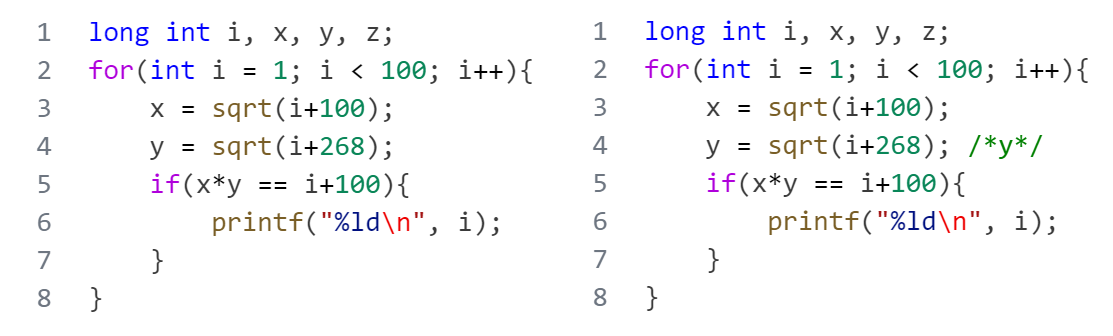
\includegraphics[scale=0.38]{types/type1}
\caption{Example of Type-1 code clone duplication.}
The example is based on the example presented by CHEN et al. \citep{litreview}. 
\label{fig:type1}
\end{figure}

\begin{figure}
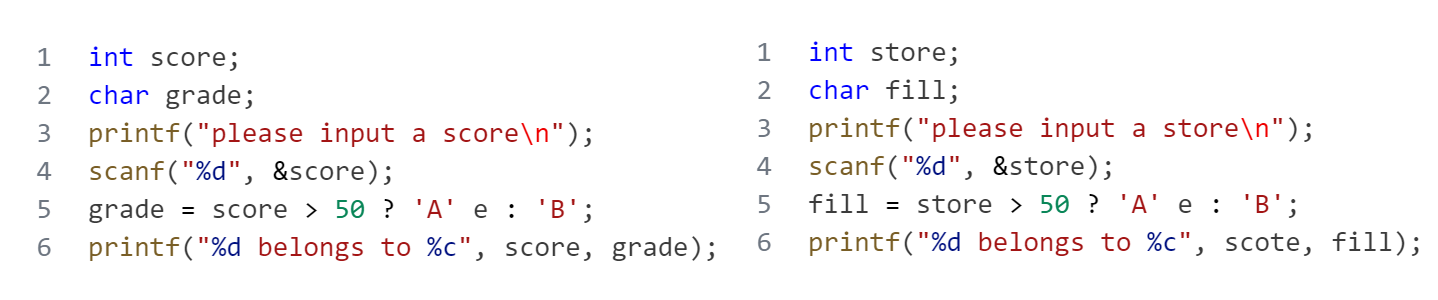
\includegraphics[scale=0.38]{types/type2}
\caption{Example of Type-2 code clone duplication.}
The example is based on the example presented by CHEN et al. \citep{litreview}. 
\label{fig:type2}
\end{figure}

\begin{figure}
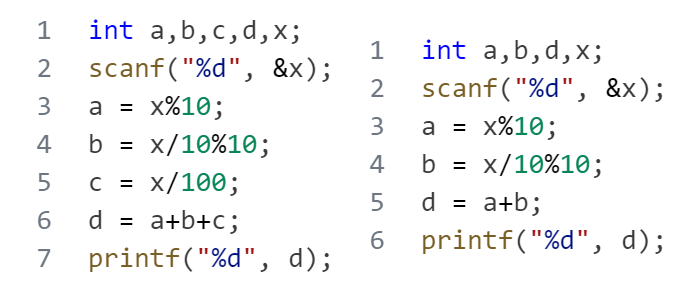
\includegraphics[scale=0.38]{types/type3}
\caption{Example of Type-3 code clone duplication.}
The example is based on the example presented by CHEN et al. \citep{litreview}. 
\label{fig:type3}
\end{figure}

\begin{figure}
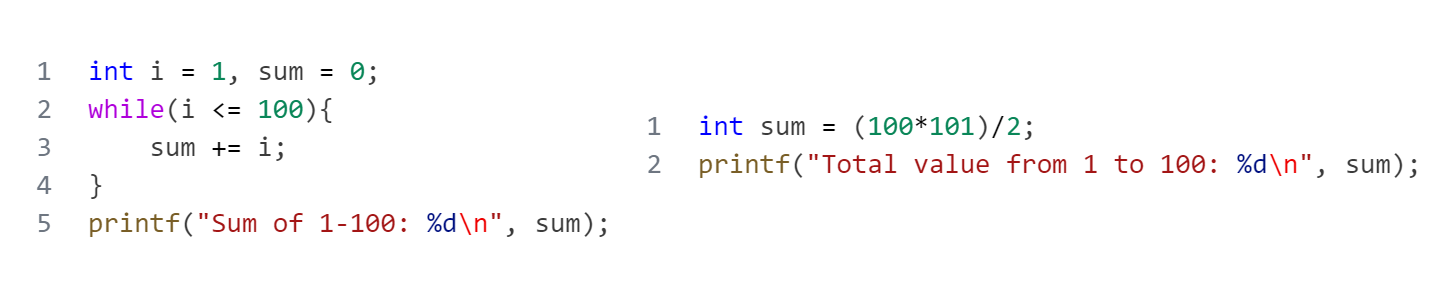
\includegraphics[scale=0.38]{types/type4}
\caption{Example of Type-4 code clone duplication.}
The example is based on the example presented by CHEN et al. \citep{litreview}. 
\label{fig:type4}
\end{figure}

\subsection{Literature approches for code clone detection}

Given the passage of time, the literature developed many techniques and methods to approach the code clone 
detection problem. For a better understanding and analysis of these approaches, the literature divided the 
research done into five methodologies given the nature of their work  \citep{litreview}, which are:

\begin{itemize}
	\item \textbf{Textual-based approaches:}  The literature review made by Chen \citep{litreview}  
	states that this methodology is the first to be investigated by the literature. This methodology line 
	is based on seeing code as a text artifact and applying textual approaches for text similarity. One 
	example of this methodology applied is the work of Roy and Cordy
	\citep{textexample},
	which uses parsing and grammar techniques to detect code clones.

	\item \textbf{Token-based approaches:} This method tries to approach the problem by seeing the code in a
	similar way to the lexical analysis of the compiling process \citep{litreview}. 
	That means doing work along the lines of recognizing constants, keywords, and other specific programming 
	language tokens, mapping variables to representations to become naming-independent, etc. One example 
	of this methodology applied is the work of Toomey et al. \citep{tokenexample} 
	to detect code clones through hashed token sequences.

	\item \textbf{Tree-based approaches:} While the token-based approach uses the lexical analysis of the 
	compiling process, the tree-based approach uses the syntax tree. The syntax tree is a data structure that 
	stores the semantic information of a code artifact concerning the programming language \citep{compiler}. 
	One example of research that uses this information to detect code clones is done by Chilowicz and Duris
	\citep{treeexample}.

	\item \textbf{Metric-based approaches:} This methodology approaches the problem by extracting metrics 
	from the code artifact and using those metrics as an embedding representation of the artifact to measure 
	similarity \citep{litreview}, similar to the famous Word2Vec work done by Mikolov et al.
	\citep{wordtovec}. Examples of metrics can be program size, number of variables, number of access to
	memory, etc. One example of this methodology applied is the work done by Kaur and Sharm
	\citep{metricexample}. 

	\item \textbf{Graph-based approaches:} Similarly to the Tree-based approaches, this methodology depends 
	heavily on an intermediate program representation, called program dependence graph (PDG) \citep{prodg}. 
	The representation stores information about the program’s control, statement, and data dependencies. 
	One example of this methodology applied is the recent work done by Liu et al. \citep{tailor},
	one of the state-of-the-art works in the field.

\end{itemize}

The state-of-the-art methods for code clone detection usually have high computational time and memory space 
usage, as well being programming language-specific approaches, which cannot be easily implemented in programming 
languages that were not used in their research \citep{litreview}. 
These are concerns for our research, and for this reason, we will use a generalist textual-based approach 
based solely on Natural Language Processing (NLP) text similarity detection methods, which we will introduce 
in Chapter \ref{cha:tool} and evaluate this approach in this work.

\subsection{Evaluating code duplication methods}

\label{subsec:codemethods}

Given the necessity to evaluate and compare approaches for code clone detection, it was developed and widely 
adopted: OJ-Clone, a dataset collected from a pedagogical online judge system \citep{ojclone},
and BigCloneBench, a dataset collected from over 25,000 Java software systems \citep{bigclonebench}. 
The existence of only two spread datasets is an open concern in literature as the limited scope of OJ-Clone 
and the problems of BigCloneBench presented by Krinke and Ragkhitwetsagul \citep{bigfail}. The BigCloneBench
is the dataset used by most of the literature works, given the limited pedagogical scope of the OJ-Clone. 

The BigCloneBench dataset does an additional split on the code clone duplications types for the Type-3,
where the dataset separated the Type-3 into three types, which are Weak Type-3 (WT3), Medium Type-3 (MT3), 
Strong Type-3 (ST3), with the WT3 being closer to the Type-4 and ST3 being closer to the Type-2 \citep{bigclonebench}.
Finally,  the BigCloneBench dataset unifies the WT3 with the T4, resulting in 6 possible outcomes of a code pair, 
which are Type-1, Type-2, Strong Type-3, Medium Type-3, Weak Type-3/Type-4, and not a duplication \citep{bigclonebench}.

To evaluate the code clone detection approaches against the datasets, the researchs compute metrics using 
the predictions made related to the instances of the dataset. There are four possible outcomes when an 
instance is predicted by a code clone detection approach, which are:

\begin{itemize}
	\begin{item}
		\textit{True positivity (TP)}: This outcome happens when the approach predicts that the instance 
		is a code clone and the instance is a code clone.
	\end{item}
	\begin{item}
		\textit{False positivity (FP)}: This outcome happens when the approach predicts that the instance 
		is a code clone, but the instance is not a code clone.
	\end{item}
		\begin{item}
		\textit{True negative (TN)}: This outcome happens when the approach predicts that the instance 
		is not a code clone and the instance is not a code clone.
	\end{item}
	\begin{item}
		\textit{False negative (FN)}: This outcome happens when the approach predicts that the instance 
		is not a code clone, but the instance is a code clone.
	\end{item}
\end{itemize}

Given the number of TP, FP, TN, and FN that resulted after an approach evaluation against a dataset,
it is possible to compute classical metrics such as Precision, Recall, and F-Score \citep{recall}.
In this work, we use the Recall metric as the code clone detection approaches usually make available 
this metric to compare themselves in contrast with the others. The Recall metric is defined by the 
following formula \citep{recall}:

$$Recall = \frac{\sum TP}{\sum TP + \sum FN }$$

Where $\sum TP$ is the number of true positives in the evaluation and $\sum FN$ is the number of 
false negatives. The Recall metric is a number between $0$ and $1$, where a value closer to $1$ is 
better, and a value closer to $0$ is worse.









